\documentclass[aspectratio=169,hyperref={pdfpagelabels=false}]{beamer}
\usepackage{helvet}
\usepackage[english]{babel}
\usepackage{pgfplots}
\usepackage{pgf}
\pgfplotsset{compat=newest}
\usepackage{booktabs}
\usepackage[T1]{fontenc}
\usepackage[utf8]{inputenc}
\usepackage{lipsum}
\usepackage{tcolorbox}
\usepackage{xcolor}
\usepackage{listings}
\usepackage{microtype}
\usepackage{float}
\usepackage{siunitx}
\usepackage{multicol}
\usepackage{hyperref}
\usepackage{dsfont}
\usepackage{caption}
\usepackage{subcaption}

% DTU colours for diagrams
% You might want to make the front/back page background colour the first colour in the plot cycle list.
\pgfplotscreateplotcyclelist{DTU}{%
dtured,         fill=dtured,        \\%
blue,           fill=blue,          \\%
brightgreen,    fill=brightgreen    \\%
navyblue,       fill=navyblue       \\%
yellow,         fill=yellow         \\%
orange,         fill=orange         \\%
grey,           fill=grey           \\%
red,            fill=red            \\%
green,          fill=green          \\%
purple,         fill=purple         \\%
}

% Table of contents (TOC) and numbering of headings
\setcounter{tocdepth}{1}    % Depth of table of content: sub sections will not be included in table of contents
\setcounter{secnumdepth}{2} % Depth of section numbering: sub sub sections are not numbered



\newcommand{\setcolor}[1]{\def\chosencolor{#1}}
\newcommand{\setdepartment}[1]{\def\department{#1}}

\usetheme{DTU}
\setbeamersize{text margin left=22mm}
\def\insertframetitle{}

\newcommand{\inserttitlepage}{

    \begin{frame}[plain]{}
        \color{white}\maketitle    
    \end{frame}

    \setbeamercolor{background canvas}{bg = white}
}

\subtitle{Error Correction in Digital Systems}
\title{Project Introduction}
\author{Tjark Petersen}
\setcolor{orange}

\usepackage{multicol}
\usepackage{siunitx}
\usepackage{biblatex}
\usepackage{xcolor}
\usepackage{hyperref}

\usepackage{etoolbox}
\makeatletter
\patchcmd{\@verbatim}
  {\verbatim@font}
  {\verbatim@font\footnotesize}
  {}{}
\makeatother

\newcommand{\sectionseperator}[1]{%

{%
\setbeamercolor{background canvas}{bg=\chosencolor}
\begin{frame}[plain]{}

        \usebeamercolor[fg]{title}

        \begin{center}
        \hspace{-3.6em}\vspace{-3.6em}{\usebeamerfont{title}\textbf{#1}\par}
        \end{center}

        
\end{frame}
}

}


\begin{document}
\inserttitlepage

\begin{frame}{Outline}

    \begin{itemize}
        \item \textbf{Recap}: How can we reliably transmit/store data via/in a noisy medium?
        \item \textbf{VHDL}: Getting friends with the compiler
        \item \textbf{Lab 1}: First part of the project
        \item \textbf{Git}: Proper project version control
    \end{itemize}

\end{frame}


\sectionseperator{Recap}

\begin{frame}{The Fundamental Problem}
    % noisy channel
    \begin{itemize}
        \item Information is sent from $X$ to $Y$ via a \textit{noisy channel}
        \item The noisy channel randomly induces bit flips in the transmitted piece of information
        \item Solution: Add redundant information in an encoder and use it in a decoder to restore the original message
        \item In Hamming code: Capture information of overlapping groups and use per group information to locate error
    \end{itemize}
    \begin{figure}
        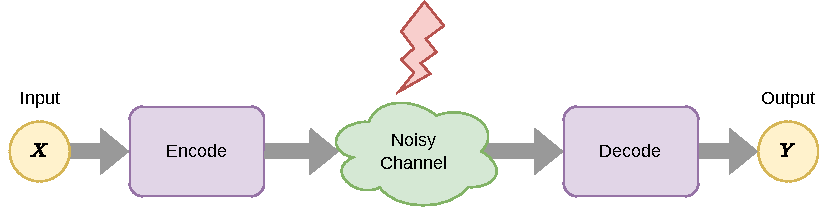
\includegraphics[width=8cm]{../introduction_slides/fig/NoisyChannel_plus_ecc.pdf}
    \end{figure}
\end{frame}

\begin{frame}{Project Plan}

    \begin{itemize}
        \item Start with some exercises on Hamming code and literature review on soft errors
        \item Implement part of an error correction capable system in VHDL
        \item Write a technical report covering the theoretical background and your implementation using LaTeX
    \end{itemize}

    \begin{figure}
        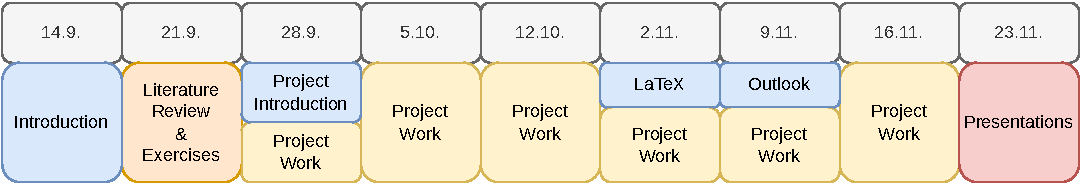
\includegraphics[width=\textwidth]{../introduction_slides/fig/CoursePlan.pdf}
    \end{figure}

\end{frame}

\sectionseperator{VHDL}

\begin{frame}{What can VHDL do for you?}

    \begin{itemize}
        \item Describe relations between signals
        \item Can be transformed by a synthesis tool to e.g. a gate or LUT circuit
        \item Design can be split into smaller entities to reduce complexity
        \item Relations between signals can be described at lower levels (e.g. boolean operators) or more abstract levels (e.g. if statements)
    \end{itemize}

\end{frame}

\begin{frame}[fragile]{Entities}
    \begin{columns}
        \begin{column}{0.64\textwidth}
\begin{verbatim}
    entity MyEntity is 
        port(
            a: in  std_logic_vector(3 downto 0);
            b: in  std_logic;
            c: out std_logic_vector(1 downto 0);
            d: out std_logic
        );
    end entity;
\end{verbatim} 

            \begin{itemize}
                \item Defines the interface to the outside world
                \item Everything inside the entity is a black box
            \end{itemize}
        \end{column}
        \begin{column}{0.35\textwidth}
            \begin{figure}
                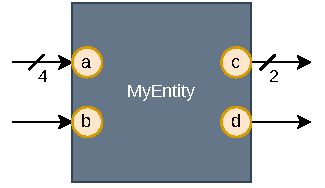
\includegraphics[width=\columnwidth]{fig/entity.pdf}
            \end{figure}
        \end{column}
    \end{columns}
\end{frame}

\begin{frame}[fragile]{Architectures}
    \begin{columns}
        \begin{column}{0.64\textwidth}
\begin{verbatim}
    architecture arch1 of MyEntity is 
        signal e: std_logic_vector(3 downto 0);
    begin
        d <= not b;
        e <= "0000" when b='1' else a;
        c <= e(2 downto 1); 
    end architecture;
\end{verbatim} 

            \begin{itemize}
                \item Defines internal signals
                \item Defines relationship between outputs, internal signals and inputs
            \end{itemize}
        \end{column}
        \begin{column}{0.35\textwidth}
            \begin{figure}
                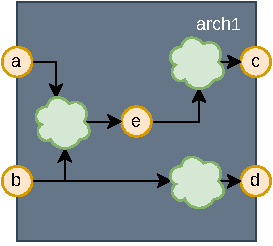
\includegraphics[width=\columnwidth]{fig/architecture.pdf}
            \end{figure}
        \end{column}
    \end{columns}
\end{frame}



\sectionseperator{Lab 1}

\begin{frame}{Lab 1}
    \begin{itemize}
        \item Implement Hamming SEC-DED encoder and decoder
        \item Send encoded message between two FPGAs and tamper with wires
    \end{itemize}
    \begin{figure}
        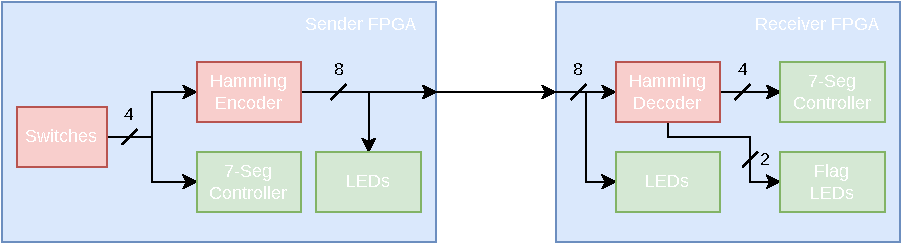
\includegraphics[width=\textwidth]{fig/Hamming_FPGA_system_block.pdf}
    \end{figure}
\end{frame}

\begin{frame}{Lab 1}
    \begin{itemize}
        \item Project repository located at: \url{https://github.com/tjarker/error-correction-project}
        \item \texttt{readme.md} contains guide
        \item \texttt{projects/} contains Vivado projects for Sender and Receiver FPGA
        \item \texttt{src/design/} contains VHDL designs
        \item \texttt{src/test/} contains VHDL testbenches
    \end{itemize}
\end{frame}

\sectionseperator{Git}

\begin{frame}{Git}

    \begin{itemize}
        \item How can multiple people collaborate on a shared code base with version control?
        \item Version control: Track changes and allow to revert them
        \item Projects are kept in repositories
        \item Created by Linus Torvalds in 2005 for Linux kernel development
        \item Widespread use especially in open-source projects
        \item Different hosting providers like GitHub, GitLab or BitBucket
    \end{itemize}

\end{frame}


\begin{frame}{Working with Git}
    \begin{itemize}
        \item \texttt{clone} a repository to get a local version on your machine
        \item Work on your local version until a feature is working
        \item \texttt{stage} relevant changed files
        \item \texttt{commit} staged files, creating a checkpoint which is the newest version of the repository
        \item \texttt{push} the commit to update the remote repository with your version
        \item \texttt{fetch} to check for new commits on the remote repository
        \item \texttt{pull} to update the local repository with the remote version
        \item \texttt{merge} remote updates with local changes
    \end{itemize}
\end{frame}

\begin{frame}{Getting Started with Lab 1}
    \begin{itemize}
        \item Install Git using the guide at \url{https://github.com/git-guides/install-git}
        \begin{itemize}
            \item For a graphical user interface install GitHub Desktop
            \item Else install a command line version
        \end{itemize}
        \item Clone \url{https://github.com/tjarker/error-correction-project}
        \begin{itemize}
            \item In Github Desktop: Add -> Clone Repository -> Enter URL
            \item The command line: Navigate to target directory and type \texttt{git clone https://github.com/tjarker/error-correction-project}
        \end{itemize}
        \item To host your own repository and collaborate in your group, find out \textcolor{blue}{\href{https://docs.github.com/en/get-started/quickstart/fork-a-repo}{how to fork}}
        \item Usually only source files are part of a Git repository 
        \begin{itemize}
            \item Take a look at the \texttt{.gitignore} file and see what is excluded from being tracked by Git
        \end{itemize} 
    \end{itemize}
\end{frame}

\sectionseperator{Ready To Start}




\end{document}